
\begin{comment}
\begin{figure*}[t]
\vspace{-0.15in}
\begin{center}
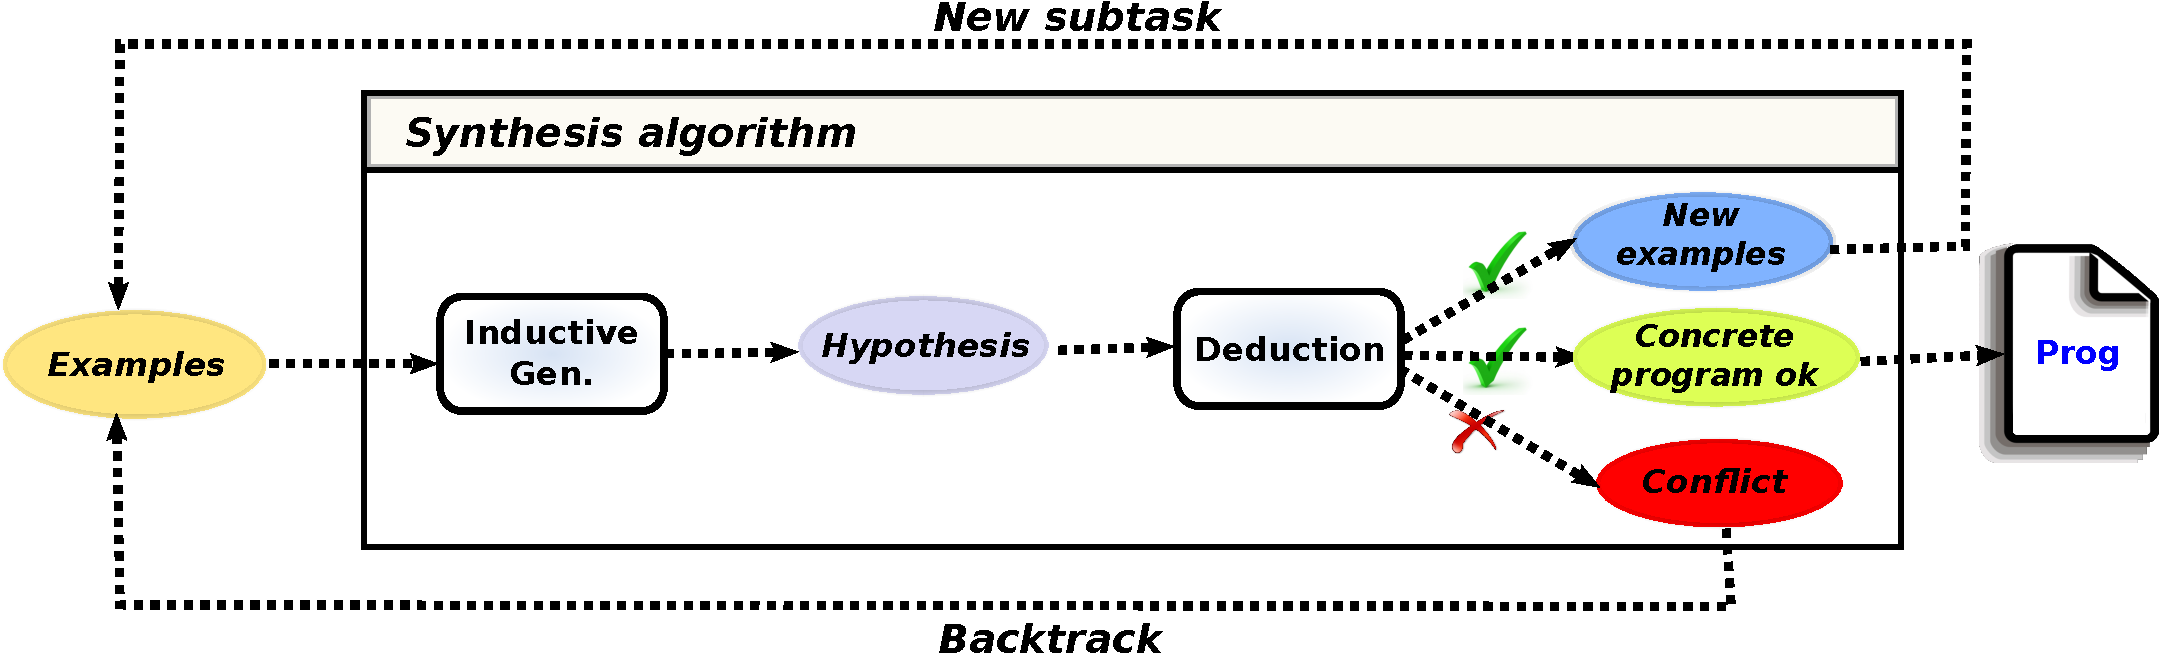
\includegraphics[scale=0.37]{overview-modified3.pdf}
\end{center}
\caption{High-level overview of our synthesis
  algorithm}\label{fig:overview}
\vspace{-0.1in}
\end{figure*}
\end{comment}

This section describes our procedure for solving the synthesis problem
from \secref{problem}.

\subsection{Algorithm architecture}\label{sec:overview}


Our synthesis procedure performs an \emph{enumerative search} that
interleaves \emph{inductive generalization} and \emph{deductive
  reasoning}. Specifically, the procedure maintains a priority queue
$Q$ of {\em synthesis subtasks} of the form $(e, f, \E)$, where $e$ is
a hypothesis, $f$ is a hole in the hypothesis, and $\E$ is a set of
examples. The interpretation of such a task is:
\begin{quote}
  Find a replacement $e^*$ for the hole $f$ such that $e^*$ satisfies
  the examples $\E$, and the program $e[e^*/f]$ obtained by
  substituting $f$ by $e^*$ satisfies the top-level input-output
  examples $\E_{in}$.
\end{quote}

The procedure iteratively processes  subtasks in the \emph{task pool} $Q$. \figref{overview} 
gives an overview of our strategy for solving each subtask $(e, f, \E)$.
First, our algorithm performs inductive generalization over  examples $\E$ to
produce a lazy stream of hypotheses $H$ about candidates $e^*$ that can  replace $f$.
As mentioned earlier, these hypotheses are
generated in a {\em type-aware} way, meaning that we %we infer the type
%$\tau$ of the target program from $\E$ and
rule out hypotheses that
are inconsistent with the inferred type $\tau$ of examples $\E$.



Next, for each hypothesis $h$ in $H$, our algorithm applies \emph{deductive
  reasoning} to check for potential {\em conflicts}. If the hypothesis
is closed, then a conflict arises if $e$ does not satisfy the
top-level (user-provided) input-output examples $\E_{in}$. 
In this case, the procedure
simply picks a new synthesis subtask from the task pool $Q$.
This corresponds to a form of \emph{backtracking} in the overall algorithm.

If the hypothesis is open, a conflict indicates that the provided
input-output examples violate a known axiom of a primitive operator
used in the hypothesis (i.e., there is {\em no way} in which the
hypothesis can be successfully completed). Upon conflict detection,
our procedure again backtracks and considers a different inductive
generalization.

If  hypothesis $h$ is open and no conflicts are found, the procedure generates new subtasks for
each hole $f$ in $h$ and uses deduction to learn new
input-output examples. In more detail, each new subtask is of the
form $(e', f^*, \E^*)$ where $e'$ is a new hypothesis, $f^*$ is a
new hole to be synthesized, and $\E^*$ is the set of inferred
input-output examples for $f^*$. This new subtask is now added to the task pool $Q$.

The procedure terminates once the search selects a subtask where the
hypothesis is closed and which does not conflict with the top-level
examples $\E_{in}$. 


 
%%%%%%%%%%%%%%%%%


 % \begin{figure}[!t]
% {\small 
%    \begin{tabbing}
%      mmm\=mmm\=mmm\=mmm\=mmm\=\kill
%      procedure {\sc Synthesize}($f, E, P, E'$):\\
    
%      \> input:  I/O examples $E$ for unknown function $f$, \\ 
%           \> \ \ \ \ \ \ \ \ \ \   program $P$ synthesized so far, and  \\
%      \> \ \ \ \ \ \ \ \ \ \ I/O examples $E'$ for the top-level synthesis problem \\
%      \> output: a program $P'$ if synthesis succeeds, $\bot$ otherwise \\
%      \> \\
%      \> (1) \> let $\tau$ := {\sc TypeInfer}$(E)$ in \\
%      \> (2) \> let $H$ := {\sc InductiveGen}($\tau$) in \\
%      \> (3) \> foreach $h \in H$: \\
%      \> (4) \> \ \ \ \ let $P'$ := $P[h/f]$ in  \\
%      \> (5) \> \ \ \ \ foreach $f^\star \in {\rm holes}(H)$: \\
%      \> (6) \> \ \ \ \ \ \ \ \  let $E^\star$ := {\sc Deduce}($h, f^*, E$) in \\
%      \> (7) \> \ \ \ \ \ \ \ \ if($E^\star = \bot$) break; \\
%      \> (8) \> \ \ \ \ \ \ \ \ let $P^\star$ := {\sc Synthesize}($E^\star, f^\star, E', P'$) in \\
%      \> (9) \> \ \ \ \ \ \ \ \ if($P^\star = \bot$) break; \\
%      \> (10) \> \ \ \ \ \ \ \ \ $P' := P[P^\star/f^\star]$ \\
%      \> (11) \> \ \ \ \ if({\sc Consistent}($P', E'$)) return $P'$ \\
%      \> (12) \> return $\bot$
%    \end{tabbing}
% } 
%    \caption{DO NOT TOUCH: Old synthesis algorithm}
%    \label{fig:algorithm}
%  \end{figure}
 
 
 % \todo{If we want to guarantee optimality, we need to change this
 % algorithm. Maybe pass a value $k$ to Synthesize and InductiveGen.
 % In that case, Synthesize and Inductive Gen also need to return an
 % integer that indicates the size of synthesized expression. }
 
 \figref{algorithm} gives pseudocode for the overall synthesis algorithm. Here, $Q$ is a \emph{priority queue} of
 tasks $(e, f, \E)$ sorted according to the cost of hypothesis $e$. In each iteration of the outer loop, we pick
 a \emph{minimum-cost} subtask $(e, f, \E)$ from task pool $Q$. Now, if $e$ is a closed hypothesis, 
 we use the
 routine {\sc Consistent} at line 5 to deductively check whether $e$ satisfies examples $\E_{in}$. If  this is the case,
$e$ must be a minimum-cost implementation consistent with $\E_{in}$; hence we return  $e$ as a solution to the synthesis problem. On the other
hand, if $e$ is not consistent with $\E_{in}$, we continue with a different candidate in the task pool $Q$.



 \begin{figure}[!t]
{\small 
%In tuples (h, f, Ex, Ex'), h is a hypothesis, f is a hole in it, Ex
%is examples for f, and Ex' is examples at top-level \\ 
\begin{algorithm}{Synthesize}{\E_{in}} 
Q \= \{ (f, f, \E) \}   \qquad \text{// $f$ is a fresh variable name }    \\
\begin{WHILE}{Q \ne \emptyset}
      \textrm{pick }(e, f, \E) \textrm{ from }Q \textrm{ such
        that }e\textrm{ has minimal cost}\\
      \begin{IF}{e~\textrm{is closed}}
           \begin{IF}{\CALL{Consistent}(e, \E_{in})} 
                  \RETURN e 
            \ELSE \textbf{continue}
           \end{IF} 
       \end{IF}\\
      \tau \= \CALL{TypeInfer}(\E) \\
      H \= \CALL{InductiveGen}(\tau) \\
      \begin{FOR}{h \in H}   
           e' \= e[h/f] \\
           \begin{IF}{e' \textrm{is closed}}    
              Q \= Q \cup \{ (e',\bot , \emptyset)  \} 
	      \ELSE 
	        \begin{FOR}{f^* \in \CALL{Holes}(e')}
                \E^* \= \CALL{Deduce}(e', f^*, \E) \\
                \textbf{if}~\E^* = \ \perp~\textbf{then break} \\
                %\begin{IF}{\E^* = \perp}\textbf{break} \end{IF} \\
                Q \= Q \cup \{ (e', f^*, \E^*) \} 
             \end{FOR}
           \end{IF}
       \end{FOR}
\end{WHILE} \\
\RETURN \perp
\end{algorithm}
} 
\vspace{-0.2in}
\caption{Synthesis procedure. %$\E_{in}$ is a set of
  %user-provided input-output examples
  }
   \label{fig:algorithm}
\vspace{-0.1in}
 \end{figure}

 Now, if $e$ is an open hypothesis, we still need to synthesize the free variable $f$ in $e$. 
 For this purpose, we use the {\sc TypeInfer} procedure at line 8 to infer 
 the type of $f$ from examples $\E$ and then call {\sc
   InductiveGen} to perform type-aware inductive generalization. % of examples $\E$.
  Suppose $H$ is a list of possible inductive generalizations for $f$. Now, we obtain a new hypothesis $e'$ by 
  replacing $f$ with a hypothesis $h \in H$. If $e'$ is closed, there are no new 
  unknowns to synthesize; hence, we add a single subtask $(e', \bot, \emptyset)$ to the task pool $Q$. 
  
  
  On the other hand, if $e'$ is  an open hypothesis, we generate new subtasks for synthesizing each hole in $e'$. Here, the procedure  {\sc Deduce} infers new examples for a specified hole $f^*$ in $e'$. 
  If a conflict is detected (i.e., $e'$ is not consistent with a known axiom), then {\sc Deduce} returns $\perp$, which
causes  backtracking from the current hypothesis. If no conflicts are detected, we add new subtasks of the form $(e', f^*, \E^*)$
to~$Q$.

 % conflicts with
 %axioms for operators (in this case, it returns $\perp$), and computes
 %new examples for a specified hole in the hypothesis.

 \begin{comment}
 Note that, in each iteration of the main loop, our synthesis algorithm picks a
 subtask $(e, f, \E)$ where the cost of $e$ is minimal among all
 available choices. We show in \secref{optimality} that this strategy
 guarantees optimality of synthesis.
\end{comment}

\subsection{Hypothesis Generation}\label{sec:ind-gen}

% As mentioned earlier, our algorithm generates two kinds of
% hypotheses: (i) concrete programs, and (ii) program skeletons with
% holes. From now on, we will refer to the first kind of hypothesis as
% a \emph{concrete hypothesis} and to the latter as an \emph{abstract
% hypothesis}. Our abstract hypotheses are drawn from a family of
% combinators that involve higher-order functions and that are
% commonly used to implement data structure transformations (e.g.,
% {\tt filter}, {\tt fold} etc.)
This section explains the hypothesis generation step of the synthesis algorithm in more detail.


The first step of inductive generalization is to decide if we
want to generate a closed or open hypothesis.  Since open hypotheses
are used to encapsulate common data structure transformation patterns,
we only introduce them when the input
examples correspond to recursive data structures. In particular, if
the inferred type of the transformation is $\tau_1 \rightarrow \tau_1$
and $\tau_1$ and $\tau_2$ are primitive types (e.g., ${\tt int}
\rightarrow {\tt int}$), then our procedure only generates closed
hypotheses.
% ~\footnote{Our current implementation also has a fixed depth limit
% beyond which it only generates concrete hypotheses.}


\begin{figure*}
{\small 
\begin{center}
\begin{tabular}{|c|l|}
\hline 
Hypothesis &  Definition of Combinator  \\ \hline
$\lambda x. \ \mathtt{map} \ f \ x$ & 
\begin{tabular}{l} 
  ${\tt map}$ \ :: $(a \rightarrow b) \rightarrow {\tt list}[a]  
  \rightarrow {\tt list}[b]$  \\
  ${\tt map}$ \ $f\ [\ ]  = [ \ ] $ \\
  ${\tt map}$ \ $f\ (x:y)  = (f \ x):({\tt map}\  y \ f) $ 
 \end{tabular}  
   \\ \hline
  $\lambda x. \ {\tt mapt} \ f \ x $ &
  \begin{tabular}{l} 
  ${\tt mapt}$ \ :: $ (a \rightarrow b) \rightarrow {\tt tree}[a] \rightarrow {\tt tree}[b]$  \\
  ${\tt mapt}$ \ $f\ {\tt tree}()  = {\tt tree}()$  \\
  ${\tt mapt}$ \ $f\ {\tt tree}(x, y) = {\tt tree}(f \ x,\ {\tt
    mapt} \ f \ y)$  \\
 \end{tabular}  \\ \hline
 $\lambda x. \ {\tt filter} \ f \ x$ & 
  \begin{tabular}{l} 
  ${\tt filter}$ \ :: $(a \rightarrow {\tt bool}) \rightarrow {\tt list}[a] \rightarrow {\tt list}[a]$  \\
  ${\tt filter}$ \ $f\ [\ ] = [ \ ] $ \\
  ${\tt filter}$ \ $(x:y)  \ f = \mathrm{if}~f \ x\ \mathrm{then} \
  x:({\tt filter}\ f \ y)  \  \mathrm{else} \  {\tt filter} \  f \ y$
 \end{tabular} 
 \\
\hline
$\lambda x. \ {\tt foldl} \ f \ e\ x$ & 
  \begin{tabular}{l} 
  ${\tt foldl}$\ :: $(b \rightarrow a \rightarrow b) \rightarrow b \rightarrow {\tt list}[a]  \rightarrow b$  \\
  ${\tt foldl}$ \ $f \ e\ [\ ]= e $ \\
  ${\tt foldl}$ \ $f\ e\ (x:y) =  {\tt foldl}  \ f \ (f \ e \ x)\ y$ \\
 \end{tabular} 
\\ \hline
$\lambda x. \ {\tt foldr} \ f \ e \ x$ & 
  \begin{tabular}{l} 
  ${\tt foldr}$\ :: $(b \rightarrow a \rightarrow b) \rightarrow b \rightarrow {\tt list}[a]  \rightarrow b$  \\
  ${\tt foldr}$ \ $f \ e\ [\ ]  = e $ \\
  ${\tt foldr}$ \ $f \ e\ (x:y) = f \ ({\tt foldr} \ f \ e\ y) \ x$ \\
 \end{tabular} 
\\  \hline 
 $\lambda x. \ {\tt foldt} \ f \ e\ x$ & 
  \begin{tabular}{l} 
  ${\tt foldt}$\ :: $({\tt list}[b] \rightarrow a \rightarrow b)
  \rightarrow b \rightarrow {\tt tree}[a] \rightarrow b$  \\
  ${\tt foldt}$ \ $f \ e\ {\tt tree}() = e$  \\
  ${\tt foldt}$ \ $f \ e\ {\tt tree}(x, y) = f \ ( {\tt map}\ (\lambda
  z. \  {\tt foldt} \ f \ e \ z)\ y) \ x$ \\
 \end{tabular}  \\
 \hline 
 
  $\lambda x. \ {\tt recl}\ f \ e\ x$ & 
  \begin{tabular}{l} 
    ${\tt recl}$\ :: $(a \rightarrow {\tt list}[a] \rightarrow b) \rightarrow b \rightarrow {\tt list}[a] \rightarrow  b$   \\
  ${\tt recl} \  f \ e\  \emptylist = \ e $  \\
  ${\tt recl}\ f \  e \ (x: y)  = \ f \  x \ y $ \\
 \end{tabular}  \\ \hline
\end{tabular}
\end{center}
}
\vspace{-0.1in}
\caption{Family of combinators from which we draw our open
  hypotheses. 
  %In the last definition,  function $f$  may refer to {\tt
   % recl}.
   } 
\label{fig:abstract-hypotheses}
\vspace{-0.1in}
\end{figure*}


The open hypotheses are drawn from the family of combinators shown in
\figref{abstract-hypotheses}. The first column of
\figref{abstract-hypotheses} shows the hypothesis which serves as our
inductive generalization, and the second column shows the definition
of the combinator used in the hypothesis. Observe that the free
variables in the first column correspond to new 
synthesis subproblems.
%For instance, if our inductive generalization is an open
%hypothesis of the form $\lambda x. \ \mathtt{map} \ f \ x$, our
%procedure must recursively synthesize an implementation for free
%variable $f$ used in this hypothesis.

Open hypothesis generation is guided by the inferred type of the
input-output examples. For instance, suppose we have the 
examples $\{ 
[\ ] \mapsto 0, [1] \mapsto 1, [1,2] \mapsto 3  \}$.
%$$
%[\ ] \mapsto 0 \qquad~~~ [1] \mapsto 1 \qquad~~~ [1,2] \mapsto 3
%$$
% \[
% \begin{array}{ccc}
%  [ \ ] & \rightarrow  & 0 & & 
% {\rm [ 1 ]} & \rightarrow & 1 \\
% {\rm [ 1, 2 ]} & \rightarrow & 3
% %[ 1 ] \rightarrow 1 
% %[1, 2] \rightarrow 3
% \end{array}
% \]
Here, since the inferred type of the transformation is $\mathtt{list}[
\mathtt{int}] \rightarrow \mathtt{int}$, our hypothesis generator
immediately rules out the first three combinators from
\figref{abstract-hypotheses} from being possible
generalizations. The use of types to guide generalization is
an important feature of our procedure and greatly helps to keep the
search space manageable (see ~\secref{eval}).

%In particular, using types to guide the
%generation of closed hypothesis is a significant performance
%improvement, as shown in Figure~\ref{fig:timing}.

If the inferred type of the input-output examples is not compatible
with any of the open hypotheses from \figref{abstract-hypotheses},
%or if the recursion depth exceeds some pre-determined threshold,
our synthesis procedure instead generates closed hypotheses. This is done by lazily
enumerating a stream of candidate expressions %(closed hypotheses) 
that
are compatible with the inferred type of the input-output
examples. The enumeration procedure generates the candidate expressions in increasing
order of cost.

Our hypothesis generator also uses a rewrite system to avoid
enumerating syntactically distinct but semantically equivalent
hypotheses. Given a candidate hypothesis $e$, this rewrite system
produces either the original hypothesis $e$ or an equivalent, but
lower-cost hypothesis $e'$. As our goal is to find a minimal-cost
program, we can safely prune $e$ from the search space in the latter
case.
For example, suppose our signature has addition as a primitive operator, 1
and 0 as constants, and the axiom $\forall x. x + 0 = 0 + x = 1$. In
this case, our rewrite system will make sure that $(1 + 0)$ is not
generated as a closed hypothesis. 

% Since the enumeration procedure is complete, whenever the rewrite
% system produces a lower-cost expression $e'$, this means that
% expression $e$ has already been explored; hence, we can safely prune
% $e$ from the search space.

% This pruning strategy greatly reduces the search space in
% practice. In particular, since our closed hypothesis generator
% recursively enumerates all expressions of type $t$ in a top-down
% fashion, pruning a single expression of type ${\rm list[int]}$
% allows our algorithm to prune a large number of expressions of type
% {\rm int}.


\begin{comment}
\todo{SC: I don't like this example too much. I'll fold this into
  the text on optimality.}

\begin{example}
  %The enumeration procedure starts with a set $I$ of expressions of
  %size 1 and a set of operators. To enumerate expressions of type
  %$\tau$, we first enumerate all expressions of type $\tau$ in
  %$I$. Next, we recursively apply operators to the expressions in $I$
  %to generate larger expressions. 
  Consider the enumeration of all expressions of type {\tt int} where
  the only expressions of size $1$ are $0, 1$, and $x$. Further,
  suppose that the only operator allowed on {\rm Int}'s is $+$. In
  this case, our procedure (with pruning) will generate the following
  stream: $0, 1, x, 1 + 1, 1 + x, x+x\dots$.
  
  
  %following stream will be generated: $0, 1, x, 0 + 0, 0 + 1, 0 + x, 1
  %+ 0, 1 + 1, 1 + x, \dots$. After pruning, the stream will be: $0, 1,
  %x, 1 + 1, 1 + x, \dots$.

  % Consider the enumeration of all expressions of type {\rm int}. As
  % part of the enumeration, we select all operators whose return
  % types unify with {\rm int} (i.e. Plus, Minus, Car, If). If the
  % operator has a polymorphic return type, we unify it with {\rm Int}
  % to get a substitution, and apply that substitution to the operator
  % type. For instance, {\rm If} is of type $bool \rightarrow a
  % \rightarrow a \rightarrow a$. Unifying $a$ with {\rm Int} returns
  % the substitution $[a: {\rm Int}]$ and applying that substitution
  % to the type of {\rm If} yields $bool \rightarrow {\rm Int}
  % \rightarrow {\rm Int} \rightarrow {\rm Int}$. Now that we have
  % operator types that are specialized for the correct return type,
  % we can search for arguments to these operators.

  % To search for operator arguments, we recursively call the
  % expression enumeration procedure to obtain streams for each
  % argument type. These streams are combined into a single stream of
  % argument lists using the composition operator defined by
  % Spivey. This process is performed for each selected operator and
  % the streams are merged to produce a stream of expressions of type
  % {\rm Int}.

  % Now it should be clearer why pruning expression streams is
  % valuable, even if it can only discard expressions that are already
  % generated. Generating an expression stream for type {\rm Int}
  % requires an expression stream for types {\rm Bool} and {\rm Int},
  % among others. Any pruning that can be performed significantly
  % reduces the total number of expressions that will be tested.
\end{example}
\end{comment}

\subsection{Inference of new examples using deduction}\seclabel{deduction}

%When the hypothesis generator produces an abstract hypothesis, our algorithm must recursively synthesize one or more unknown %functions that are used in the program skeleton. Furthermore, since the {\sc Synthesize} procedure from %Figure~\ref{fig:algorithm} requires input-output examples, we must construct new  examples characterizing the unknown %functions used in the skeleton. This task is accomplished using the {\sc Deduce} procedure used at line 6 of the {\sc %Synthesize} algorithm in Figure~\ref{fig:algorithm}. In this section, we  describe the core ideas underlying the {\sc Deduce} %procedure for generating new input-output examples characterizing the recursive subproblems.

We now explain the {\sc Deduce} procedure used in the synthesis algorithm
from Figure~\ref{fig:algorithm}.
Recall that {\sc Deduce} is used for 
inferring new input-output examples and detecting conflicts.
The deduction procedure used in our synthesis algorithm is \emph{sound} but \emph{incomplete}. In this context, we
define {soundness} and {completeness} as follows:

\begin{definition}{\bf (Soundness of deduction)} Let $\E$ be a set of
  input-output examples, and let $h$ be a hypothesis that is an
  inductive generalization of $\E$.  The {\sc Deduce} procedure is
  sound, if for every unknown $f$ in $h$, whenever {\sc Deduce}($h, f,
  \E$) = $\E'$ and the synthesis problem defined by $\E'$ and $f$ does
  not have a solution, then the synthesis problem defined by $\E$ and
  $h$ also does not have a solution.
\end{definition}

In other words, the deduction procedure is sound if the non-existence
of a solution to any  synthesis subtask implies the
non-existence of a solution to the original problem. Hence, soundness
implies that deduction will never cause our synthesis
procedure to reject a valid open hypothesis. However, since our
deduction procedure is not complete, the existence of a solution to
all  synthesis subtasks does not imply the existence of a
solution to the original problem. More technically, we define
{completeness} as follows:

\begin{definition}{\bf (Completeness of deduction)} Let $\E$ be a set of
  examples, and let $h$ be a hypothesis that is an inductive
  generalization of $\E$.  The completeness of {\sc Deduce} means that,
  if the synthesis problem defined by $\E, h$ does not have a solution,
  then there exists some unknown $f$ in $h$ such that (i) {\sc Deduce}($h,
  f, \E$) = $\E'$ and (ii) the synthesis problem defined by $\E', f$ does not
  have a solution.
\end{definition}

A consequence of incompleteness is that our synthesis procedure must
check that a closed hypothesis is consistent with the
user-provided example set $\E_{in}$. This is done in line 5 of the
{\sc Synthesize} procedure in Figure~\ref{fig:algorithm}.


\begin{figure*}
{\small 
\[
\begin{array}{c}
\irule{
\begin{array}{c}
\E = \bigcup_{1 \leq i \leq n} \{ [a_{i1}, \ldots, a_{ig(i)}] \mapsto  [b_{i1}, \ldots, b_{ih(i)}] \} \\
\exists i. (1 \leq i \leq n \land g(i) \neq h(i))
 \end{array}
}{\E, \lambda x. \ {\tt map} \ f\ x \vdash f: \bot } \qquad \qquad 

\irule{
\begin{array}{c}
\E = \bigcup_{1 \leq i \leq n} \{ [a_{i1}, \ldots, a_{ig(i)}] \mapsto  [b_{i1}, \ldots, b_{ih(i)}] \} \\
\exists i, j, k, m. \left ( 
\begin{array}{c} 
1 \leq i \leq n \land 1 \leq j \leq n \land 1 \leq k \leq g(i) \land \\ 1 \leq m \leq h(j)
\land a_{ik}  =  a_{jm} \land b_{ik} \neq b_{jm})
\end{array}
\right )
 \end{array}
}{\E, \lambda x. \ {\tt map} \ f \ x\vdash f: \bot } \\ \ \\ 

\irule{
\begin{array}{c}
\E = \bigcup_{1 \leq i \leq n} \{ [a_{i1}, \ldots, a_{ig(i)}] \mapsto  [b_{i1}, \ldots, b_{ig(i)}] \} \\
\E' = \bigcup_{1 \leq i \leq n} \{ a_{i1} \mapsto b_{i1}, \ldots  a_{ig(i)} \mapsto b_{ig(i)}\} \\
 ( (a, b) \in \E' \land (a', b') \in \E' \land a = a') \Rightarrow b = b'
 \end{array}
}{\E, \lambda x. \ {\tt map} \ f\ x \vdash f: \E'} \qquad \qquad  

\irule{
\begin{array}{c}
\E = \bigcup_{1 \leq i \leq n} \{ s_i \mapsto t_i \} \\
\exists i. (1 \leq i \leq n \land s_i \not\simeq t_i) \\
 \end{array}
}{\E, \lambda x. \ {\tt mapt} \ f\ x \vdash f: \bot } \\ \ \\  

\irule{
\begin{array}{c}
\E = \bigcup_{1 \leq i \leq n} \{ s_i \mapsto t_i \} \\
\exists i, j, k, m. \left ( 
\begin{array}{c} 
1 \leq i \leq n \land 1 \leq j \leq n \land 1 \leq k \leq {\rm size}(s_i) \land \\ 1 \leq m \leq {\rm size}(t_i)
\land s_{ik} = s_{jm} \land t_{ik} \neq t_{jm})
\end{array}
\right )
 \end{array}
}{\E, \lambda x. \ {\tt mapt} \ f \ x \vdash f: \bot } \qquad 

\irule{
\begin{array}{c}
\E = \bigcup_{1 \leq i \leq n} \{ s_i \mapsto t_i \} \qquad  k = {\rm size}(s_i) = {\rm size}(t_i) \\
\E' = \bigcup_{1 \leq i \leq n} \{ s_{i1} \mapsto t_{i1}, \ldots  s_{ik} \mapsto t_{ik}\} \\
 ( (a, b) \in \E' \land (a', b') \in \E' \land a = a') \Rightarrow b = b'
 \end{array}
}{\E, \lambda x. \ {\tt mapt} \ f \ x \vdash f: \E'} \\  \ \\

\irule{
\begin{array}{c}
\E = \bigcup_{1 \leq i \leq n} \{ [a_{i1}, \ldots, a_{ig(i)}] \mapsto  [b_{i1}, \ldots, b_{ih(i)}]  \} \\
\exists i. (1 \leq i \leq n \ \land \ h(i) > g(i)) 
\end{array}
}
{\E, \lambda x. \ {\tt filter} \ f \ x \vdash f: \bot}
\qquad \qquad 
\irule{
\begin{array}{c}
\E = \bigcup_{1 \leq i \leq n} \{ [a_{i1}, \ldots, a_{ig(i)}] \mapsto  [b_{i1}, \ldots, b_{ih(i)}]  \} \\
\exists i. \exists j. 1 \leq i \leq n \land 1 \leq j \leq g(i) \land \forall k. (k \geq j \Rightarrow b_{ij} \neq a_{ik})
\end{array}
}
{\E, \lambda x. \ {\tt filter} \ f \ x \vdash f: \bot}
\\ \ \\ 
\irule{
\begin{array}{c}
\E = \bigcup_{1 \leq i \leq n} \{ [a_{i1}, \ldots, a_{ig(i)}] \mapsto  [b_{i1}, \ldots, b_{ih(i)}]  \} \qquad \qquad 
\forall i. 1 \leq i \leq n \mapsto h(i) \leq g(i) \\
\forall (A \mapsto B) \in \E. \forall b_i \in B. \exists a_j \in A. (j \geq i \land b_i = a_j) \\
\E_T = \{ x \mapsto {\rm true} \ | \ x \in A \land x \in B \land A \mapsto B \in \E\} \qquad \qquad 
\E_F = \{ x \mapsto {\rm false} \ | \ x \in A \land x \not \in B \land A \mapsto B \in \E\} 
\end{array}
}
{\E, \lambda x. \ {\tt filter} \ f \ x \vdash f: \E_T \cup \E_F}

\end{array}
\]
}
\vspace{-0.1in}
\caption{Deductive reasoning for {\tt map},  {\tt mapt}, and {\tt filter}}\label{fig:deduce-map-filter}
\vspace{-0.1in}
\end{figure*}

We  now describe the deduction engine underlying our procedure as
inference rules of the form $
\E, h \vdash f: \E' $.
The meaning of this judgment is that, if $\E$ is a set of input-output
examples with inductive generalization $h$, then $\E'$ is a new set of
input-output examples for unknown $f$ used in expression $h$. Here,
$\E'$ may also be $\bot$, indicating that a conflict is detected and
that the subproblem defined by $f$ does not have a
solution. Note that the soundness of deduction implies that, if $\E, h
\vdash f: \bot$, then $h$ cannot be a correct inductive generalization
for examples $\E$.

%Since the inferred examples depend on the ``shape'' of  the abstract hypothesis, we have a custom deduction procedure for each different inductive generalization shown in Figure~\ref{fig:abstract-hypotheses}. For instance, 
%

Figure~\ref{fig:deduce-map-filter} shows the deductive reasoning
performed for hypotheses involving the {\tt map}, {\tt mapt} and {\tt
  filter} combinators. The first three rules in
Figure~\ref{fig:deduce-map-filter} concern hypotheses involving {\tt
  map}.  Specifically, the first rule deduces a conflict if $\E$
contains an input-output example of the form $A \mapsto B$ such
that $A$ and $B$ are lists but their lengths are not equal.
Similarly, the second rule deduces $\bot$ if $\E$ contains a pair of
input-output examples $A \mapsto B$ and $A' \mapsto B'$ such
that $A_i = A'_j$ but $B_i \neq B'_j$. Since function $f$ provided as
an argument to the {\tt map} combinator must produce the same output
for a given input, the existence of such an input-output example
indicates the hypothesis must be incorrect. Finally, the third rule in
Figure~\ref{fig:deduce-map-filter} shows how to deduce new examples
for $f$ when no conflicts are detected. Specifically, for an
input-output example of the form $A \mapsto B$ where $A$ and $B$
are lists, we can deduce examples $A_i \mapsto B_i$ for function
$f$.




\begin{example}
  Consider the input-output examples $[1, 2] \mapsto [2, 3]$ and $[2,
  4] \mapsto [3, 5]$ and the hypothesis $\lambda x. \ {\tt map} \ f \
  x$. Using the third rule from Figure~\ref{fig:deduce-map-filter}, we
  deduce the following new examples for $f$: $\{ 1 \mapsto 2, 2
  \mapsto 3, 4 \mapsto 5 \}$.
\end{example}

\begin{example}
  Consider the input-output examples $[1] \mapsto [1]$ and $[2,1,4]
  \mapsto [2, 3, 7]$ and the hypothesis $\lambda x. \ {\tt map} \ f \
  x$.  We can derive a conflict using the second rule of
  Figure~\ref{fig:deduce-map-filter} because $f$ maps  input $1$ to
  two different values $1$ and $3$.
  % This reasoning is sound since no instantiation of the hypothesis
  % can result in an expression that is consistent with the provided
  % examples.
\end{example}

Since the rules for {\tt mapt} are  similar to those for {\tt map},
 we do not explain them in detail. We use the notation $s_i \not \simeq t_i$ to indicate that trees $s_i$
and $t_i$ have incompatible ``shapes''.

%The second rule is almost identical to the second rule for {\tt map}; for list examples, elements are numbered by index %whereas for trees, elements are numbered in breadth-first order. Similarly, the third rule for {\tt mapt} shows how to deduce $new examples in the same manner as they are deduced for {\tt map}.

The last three rules of Figure~\ref{fig:deduce-map-filter} describe
the deduction process for the {\tt filter} combinator. Since $\lambda
x. {\tt filter} \ f \ x$ removes those elements of $x$ for which
$f(x)$ evaluates to false, the length of the output list cannot be
greater than that of the input list. Hence, the first rule for {\tt
  filter} derives a conflict if there exists an example $A \mapsto B$
such that the length of list $B$ is greater than the length of list
$A$.  Similarly, the second rule for {\tt filter} deduces $\bot$ if
there is some element in list $B$ that does not have a corresponding
element in list $A$.  If no conflicts are detected, the last rule of
Figure~\ref{fig:deduce-map-filter} infers input-output examples for
$f$ such that an element $x$ is mapped to true if and only if it is
retained in output list~$B$.

\begin{example}
  Consider the input-output example $[1, 2] \mapsto [1, 2, 1, 2]$ and
  the hypothesis $\lambda x. \ {\tt filter} \ f \ x$. Our procedure
  deduces a conflict using the first rule for {\tt filter}.
\end{example}

\begin{example}
  Consider the input-output example $[1, 2, 3] \mapsto [1, 3, 2]$ and
  the hypothesis $\lambda x. \ {\tt filter} \ f \ x$. This time, our
  procedure deduces $\bot$ using the second rule for {\tt filter}.
\end{example}

\begin{example}
  Consider the examples $[1, 2, 3] \mapsto [2]$ and $[2,
  8] \mapsto [2, 8]$ and the hypothesis $\lambda x. \ {\tt filter} \ f
  \ x$. Using the last rule of Figure~\ref{fig:deduce-map-filter}, we
  derive the following examples for $f$: $\{ 1\mapsto \false, 2
  \mapsto \true, 3 \mapsto \false, 8 \mapsto \true \}$.
\end{example}

% \todo{Question for Jack: Should we not have another inference rule
% that deduces a conflict if $f(i)$ is mapped to
% both %true and false? If so, can you add this as an inference rule along with an explanation?}

We now describe the deductive reasoning performed for the {\tt
  foldl} and {\tt foldr} combinators (we collectively refer to these
operators as {\tt fold}).  Consider a hypothesis of the form
$\lambda x. \ {\tt fold} \  f \ e \ x$ and suppose we want to learn new
input-output examples characterizing $f$. We have found that deducing
new examples for $f$ in a sound and scalable way is only possible if the
expression $e$ is a constant, as oppposed to a function of
$x$. Therefore, our procedure generates two separate hypotheses
involving {\tt fold}:

\begin{enumerate}
\item $\lambda x. \ {\tt fold}  \ f \ c \ x$  where $c$ is a constant
\item $\lambda x. \ {\tt fold}  \ f \ e\ x$  where $e$ is an arbitrary expression.
\end{enumerate}

Our deduction engine can make inferences and generate useful examples
only for case (1).  The second case relies on enumerative search,
which is possible even without examples.  As new examples can prune
the search space significantly, synthesis is more likely to be
efficient in case (1), and we always try the first hypothesis before
the second one. In what follows, we discuss the inference rules for
{\tt fold} under the assumption that it has a constant base case.

Figure~\ref{fig:deduce-fold} describes the deduction process for
combinators involving {\tt foldl}, {\tt foldr} and {\tt rec} using set
inclusion constraints. Specifically, the set $\E'$ in these rules
denotes the smallest set satisfying the generated
constraints. Consider the first two rules of
Figure~\ref{fig:deduce-fold}. By the first rule, if there are two
input-output examples of the form $[\ ] \mapsto b$ and $[~] \mapsto
b'$ such that $b \neq b'$, this means that we cannot synthesize the
program using a fold operator with a constant base case; hence we
derive $\bot$. Otherwise, if there is an example $[~] \mapsto b$, we
infer the initial seed value for {\tt fold} to be $b$.

\begin{comment}
  While the deductive reasoning performed for the {\tt map} and {\tt
    filter} combinators is both sound and complete, the inference
  rules shown in Figure~\ref{fig:deduce-fold} for the {\tt fold} and
  general recursion ({\tt rec}) combinators are sound but incomplete.
  Figure~\ref{fig:deduce-fold} describes the deduction process for
  these combinators using set inclusion constraints. Specifically, the
  set $E'$ in these rules denotes the smallest set satisfying the
  generated constraints.

However, the inference rules for folds are only sound when the base
case for the fold is constant. If the base case is known to be
non-constant, examples can be inferred for $e$, but not for $f$. It is
not correct to assume that, because all provided examples have a
constant base case, the base case is constant in general. While it is
safe to assume a fixed base and deduce examples, in general we are
searching for a base case. 
\end{comment}


Let us now consider the  third rule (i.e., {\tt foldr}), and suppose  we have an example
$E_1: \ [a_1, \ldots, a_n] \mapsto b$ and another example $E_2: \ \ {\rm [}a_2, \ldots, a_n{\rm ]} \mapsto b' $.
%the following pair of input-output examples:
%\[
%\begin{array}{ll}
%E_1: \ \ [a_1, \ldots, a_n] \mapsto b \ \ \ & \ \ \  
%E_2: \ \ {\rm [}a_2, \ldots, a_n{\rm ]} \mapsto b' 
%\end{array}
%\]
Now, observe the following equivalences:
\[
\begin{array}{ll}
 {\tt foldr} \  f \ y\ [a_1, \ldots, a_n]  & \\
 \ \ \ \equiv   f \  ({\tt foldr} \ f \ y\ \ [a_2, \ldots, a_n]) \ a_1 & {\rm (def. \ of \  {\tt foldr})} \\
 \ \ \ \equiv f \   b' \ a_1  & {\rm (from}\  E_2) \\
 \ \ \ \equiv b & {\rm (from} \ E_1)
\end{array}
\]
Since we have  $f \ b' \ a_1 = b$, it is sound to deduce the input-output example $( b', a_1) \mapsto b$ for the unknown function $f$.

As shown in the fourth rule, we  can apply similar reasoning to {\tt foldl}. Suppose we have the following  examples:
\[
\begin{array}{ll}
E_1': \ \ [a_1, \ldots, a_n] \mapsto b  \ \ \  &  \ \ \ 
E_2': {\rm [}a_1, \ldots, a_{n-1}{\rm ]} \mapsto b' 
\end{array}
\]
We can again expand the recursive definition of {\tt foldl} to obtain the following equivalences:
\[
\begin{array}{ll}
 {\tt foldl}\ f \ y\ \ [a_1, \ldots, a_n]  & \\
 \ \ \ \equiv    f \ a_n\ ({\tt foldl} \ f \ y\ \  [a_1, \ldots, a_{n-1}])   & {\rm (property \ of \  {\tt foldl})} \\
 \ \ \ \equiv f \   a_n \ b'  & {\rm (from}\  E_2') \\
 \ \ \ \equiv b & {\rm (from} \ E_1')
\end{array}
\]
Hence, we can   infer the input-output example $(a_n, b') \mapsto b$ for function $f$. However, as illustrated by the following example, these inference rules are not complete.

\begin{figure}
{\small 
\[
\begin{array}{c}
  \irule{([] \mapsto b)  \  \in \E,  \ \ ([] \mapsto b')  \  \in \E,  \ \ b \neq b' }
  {\E, \lambda x. \ {\tt fold}\ f \ c\ x \vdash c: \bot} \\ \ \\ 
  \irule{ \ ([\ ] \mapsto b) \in \E}
  {\E, \lambda x. \ {\tt fold}\ f \ c\ x \vdash c: \{ b \}} \\ \ \\
  %\land E,
   % \lambda x. \ {\tt foldr} \ x \ f \ e \vdash e: E'} \\ \ \\
  \irule{
    \begin{array}{c}
     % (([\ ] \mapsto b) \in E \land ([\ ] \mapsto b') \in E) \Rightarrow b = b' \\
      ([a_1, \ldots, a_n] \mapsto b) \in \E \\
      ([a_2, \ldots, a_n] \mapsto b') \in \E \\
    \end{array}
  }{\E, \lambda x. \ {\tt foldr}\ f \ c\ x \vdash f: ((b', a_1) \mapsto b) \in \E'} \\ \ \\
  \irule{
    \begin{array}{c}
      %(([\ ] \mapsto b) \in E \land ([\ ] \mapsto b') \in E) \Rightarrow b = b' \\
      ([a_1, \ldots, a_n] \mapsto b) \in \E  \\
      ([a_1, \ldots, a_{n-1}] \mapsto b') \in \E \\
    \end{array}
  }{\E, \lambda x. \ {\tt foldl} \ f \ c\ x \vdash f: ((a_n, b') \mapsto b) \in \E'} \\ \ \\
  \irule{({\rm tree}() \mapsto b)  \  \in \E,  \ \ ({\rm tree}() \mapsto b')  \  \in \E,  \ \ b \neq b' }
  {\E, \lambda x. \ {\tt foldt}  \ f \ c\ x \vdash c: \bot} \\ \ \\ 
  \irule{ ({\rm tree}() \mapsto b) \in \E} 
  {\E, \lambda x. \ {\tt foldt}  \ f \ c \ x\vdash c: \{b\}} \\ \ \\

  \irule{
    \begin{array}{c}
     % (({\rm tree}() \mapsto b) \in E \land ({\rm tree}() \mapsto b') \in E) \Rightarrow b = b' \\
      {\rm tree}(a, [b_1, \ldots, b_n]) \mapsto c \in \E \\
      \forall i. (1 \leq i \leq n \Rightarrow (b_i \mapsto c'_i \in \E)) \\
    \end{array}
  }{\E, \lambda x. \ {\tt foldt} \ f \ c \ x\vdash f: ([c'_1, \ldots, c'_n], a) \mapsto c) \in \E'} \\ \ \\

  \irule{
    ( x:xs \mapsto b)  \in  \E
  }
  {\E, \lambda x. {\tt recl} \ f \ e \ x\vdash f: ((x, xs) \mapsto b) \in \E' }
\end{array}
\]
}
\vspace{-0.1in}
\caption{Deduction for {\tt fold} and general
  recursion.}\label{fig:deduce-fold}
  \vspace{-0.1in}
\end{figure}


\begin{example}
Consider the hypothesis $\lambda x. \ {\tt foldl} \ f \ y \ x$, and the following input-output examples provided by the user:
\[
\begin{array}{lll}
\emptylist \mapsto  0 & 
\mylist{1}  \mapsto  1 &
\mylist{1, 2}  \mapsto  3 \\
\mylist{2, 3} \mapsto 5 & 
\mylist{1, 2, 3} \mapsto 6 & 
\mylist{2,3,5} \mapsto 10
\end{array}
\]
Using the inference rules from Figure~\ref{fig:deduce-fold}, we infer the following input-output examples for $f$:
\[
(1, 0)  \mapsto 1, \ \ \ (2, 1) \mapsto 3, \ \ \  (3, 3) \mapsto 6, \ \ \ (5, 5) \mapsto 10
\]
Observe that  there is information provided by   $\mylist{2, 3} \mapsto 5 $ that is not captured by the inferred examples for~$f$.
\end{example}

The next three rules for {\tt foldt} are very similar to {\tt foldl} and {\tt foldr}; hence, we do not discuss them in detail.
The last rule in Figure~\ref{fig:deduce-fold} infers input-output examples for  function $f$ used in the general recursion combinator. Recall from Figure~\ref{fig:abstract-hypotheses} that, given an input list of the form $x:xs$, the general recursion combinator applies function $f$ to pair $(x, xs)$. Hence, for any input example of the form $[a_1, \ldots, a_n] \mapsto b$, we can deduce the example $(a_1, [a_2, \ldots, a_n]) \mapsto b$ for unknown function $f$.


\begin{comment}

\subsection{Extensions}
%\subsubsection{Example scopes}
\todo{I don't entirely understand this discussion. I think we need to
elaborate on this some more. --Isil}
In the implementation, IO examples are not the entire story. Given an
unknown function $f^*$, each example for $f^*$ is attached to a scope,
which contains value bindings that are accessible to the unknown
function. Consider the hypothesis $\lambda\ x.\ ${\tt map}$\ f^*\ x$
and the example $[1, 2] \mapsto [3, 4]$. When we deduce examples
for $f^*$, each example will be associated with the scope $\{x:[1,
2]\}$. When generalizing $f^*$, values in scope are considered in
addition to function arguments as possible inputs to a combinator. The
scope is considered to be part of the ``input'' side of the example,
so when comparing the left hand sides of two examples, the scopes are
compared as well as the inputs.

This has implications for the deduction rules. In particular, given
examples $a_1 \mapsto b_1$ and $a_2 \mapsto b_2$ and scopes
$s_1$ and $s_2$, we derive a conflict if and only if $a_1 = a_2 \land
s_1 = s_2 \land b_1 \neq b_2$.

\subsubsection{Search strategies}
When performing exhaustive search, we use iterative deepening to
reduce the memory cost of breadth-first search. When performing
exhaustive search for multiple open hypotheses, we need to search up
to some depth $n$ for each hypothesis before moving on to depth $n +
1$. We are using breadth-first search to enumerate closed
expressions, which takes up a significant amount of memory for the
search state. Rather than maintain the search state for each hypothesis
and switch between them, the search is restarted at each depth. This
is a tradeoff between runtime and memory use, and allows us to search
to higher depths without running out of memory.
\end{comment}
%\begin{enumerate}
%\item Maybe the termination issue and why we have to switch to exhaustive search at some point, but I am not sure if it fits here. Another possibility is to add the termination discussion at the end of Section 3.3
%\end{enumerate}

%%% Local Variables: 
%%% mode: latex
%%% TeX-master: "pldi"
%%% End: 



\subsection{Optimality of synthesis}\seclabel{optimality}

Now we show that  procedure {\sc Synthesize} from Figure~\ref{fig:algorithm} correctly solves the
synthesis problem defined in \secref{problem}.

\begin{theorem}
If {\sc Synthesize} returns program $e$ on  examples
$\E$, then  $e$ is a minimal-cost closed program that satisfies~$\E$.
\end{theorem}

\begin{proof} 
The program $e$ is guaranteed to be closed and satisfy the
input-output examples by lines 4-6 in the procedure.

We prove  optimality of $e$ by contradiction. Assume  there is
a closed  $e'$ such that $e \ne e'$, $\C(e') < \C(e)$ and $e'$
satisfies $\E$.
Consider the point  in time when {\sc Synthesize} picks a task of the form
$(e, f^*, \E^*)$ out of the task pool $Q$.
A task of the form $(e', f', \E')$ cannot be  in $Q$ at this
time or at any point of time until this point.  Otherwise, because of
line 3, {\sc Synthesize} would have picked $(e', f',\E')$ and returned~$e'$.

However, $Q$ must, at this point, contain an open hypothesis $h$ whose
free variables can be instantiated to produce $e'$. This is because the
pruning mechanisms in {\sc Synthesize} are sound; as a result, the
procedure does not rule out hypotheses from which satisfactory
programs can be generated.

We know that $\C(h) \ge \C(e)$; otherwise {\sc Synthesize} would have
picked the task involving $h$ in this loop iteration. However, note
that in our cost model (\secref{problem}), primitive operators and
constants have positive costs and free variables have cost 0. Thus, any
program of form $h[h'/f]$ must  have strictly higher cost
than $h$. This means that $C(e') > C(h)$, which implies  $C(e') >
C(e)$. This is a contradiction.
\end{proof}
